% Generated by Sphinx.
\def\sphinxdocclass{report}
\documentclass[letterpaper,10pt,english]{sphinxmanual}
\usepackage[utf8]{inputenc}
\DeclareUnicodeCharacter{00A0}{\nobreakspace}
\usepackage{cmap}
\usepackage[T1]{fontenc}
\usepackage{babel}
\usepackage{times}
\usepackage[Bjarne]{fncychap}
\usepackage{longtable}
\usepackage{sphinx}
\usepackage{multirow}


\title{Cavro XP3000 GUI Documentation}
\date{July 17, 2014}
\release{1.0}
\author{Nikos Koukis}
\newcommand{\sphinxlogo}{}
\renewcommand{\releasename}{Release}
\makeindex

\makeatletter
\def\PYG@reset{\let\PYG@it=\relax \let\PYG@bf=\relax%
    \let\PYG@ul=\relax \let\PYG@tc=\relax%
    \let\PYG@bc=\relax \let\PYG@ff=\relax}
\def\PYG@tok#1{\csname PYG@tok@#1\endcsname}
\def\PYG@toks#1+{\ifx\relax#1\empty\else%
    \PYG@tok{#1}\expandafter\PYG@toks\fi}
\def\PYG@do#1{\PYG@bc{\PYG@tc{\PYG@ul{%
    \PYG@it{\PYG@bf{\PYG@ff{#1}}}}}}}
\def\PYG#1#2{\PYG@reset\PYG@toks#1+\relax+\PYG@do{#2}}

\expandafter\def\csname PYG@tok@gd\endcsname{\def\PYG@tc##1{\textcolor[rgb]{0.63,0.00,0.00}{##1}}}
\expandafter\def\csname PYG@tok@gu\endcsname{\let\PYG@bf=\textbf\def\PYG@tc##1{\textcolor[rgb]{0.50,0.00,0.50}{##1}}}
\expandafter\def\csname PYG@tok@gt\endcsname{\def\PYG@tc##1{\textcolor[rgb]{0.00,0.27,0.87}{##1}}}
\expandafter\def\csname PYG@tok@gs\endcsname{\let\PYG@bf=\textbf}
\expandafter\def\csname PYG@tok@gr\endcsname{\def\PYG@tc##1{\textcolor[rgb]{1.00,0.00,0.00}{##1}}}
\expandafter\def\csname PYG@tok@cm\endcsname{\let\PYG@it=\textit\def\PYG@tc##1{\textcolor[rgb]{0.25,0.50,0.56}{##1}}}
\expandafter\def\csname PYG@tok@vg\endcsname{\def\PYG@tc##1{\textcolor[rgb]{0.73,0.38,0.84}{##1}}}
\expandafter\def\csname PYG@tok@m\endcsname{\def\PYG@tc##1{\textcolor[rgb]{0.13,0.50,0.31}{##1}}}
\expandafter\def\csname PYG@tok@mh\endcsname{\def\PYG@tc##1{\textcolor[rgb]{0.13,0.50,0.31}{##1}}}
\expandafter\def\csname PYG@tok@cs\endcsname{\def\PYG@tc##1{\textcolor[rgb]{0.25,0.50,0.56}{##1}}\def\PYG@bc##1{\setlength{\fboxsep}{0pt}\colorbox[rgb]{1.00,0.94,0.94}{\strut ##1}}}
\expandafter\def\csname PYG@tok@ge\endcsname{\let\PYG@it=\textit}
\expandafter\def\csname PYG@tok@vc\endcsname{\def\PYG@tc##1{\textcolor[rgb]{0.73,0.38,0.84}{##1}}}
\expandafter\def\csname PYG@tok@il\endcsname{\def\PYG@tc##1{\textcolor[rgb]{0.13,0.50,0.31}{##1}}}
\expandafter\def\csname PYG@tok@go\endcsname{\def\PYG@tc##1{\textcolor[rgb]{0.20,0.20,0.20}{##1}}}
\expandafter\def\csname PYG@tok@cp\endcsname{\def\PYG@tc##1{\textcolor[rgb]{0.00,0.44,0.13}{##1}}}
\expandafter\def\csname PYG@tok@gi\endcsname{\def\PYG@tc##1{\textcolor[rgb]{0.00,0.63,0.00}{##1}}}
\expandafter\def\csname PYG@tok@gh\endcsname{\let\PYG@bf=\textbf\def\PYG@tc##1{\textcolor[rgb]{0.00,0.00,0.50}{##1}}}
\expandafter\def\csname PYG@tok@ni\endcsname{\let\PYG@bf=\textbf\def\PYG@tc##1{\textcolor[rgb]{0.84,0.33,0.22}{##1}}}
\expandafter\def\csname PYG@tok@nl\endcsname{\let\PYG@bf=\textbf\def\PYG@tc##1{\textcolor[rgb]{0.00,0.13,0.44}{##1}}}
\expandafter\def\csname PYG@tok@nn\endcsname{\let\PYG@bf=\textbf\def\PYG@tc##1{\textcolor[rgb]{0.05,0.52,0.71}{##1}}}
\expandafter\def\csname PYG@tok@no\endcsname{\def\PYG@tc##1{\textcolor[rgb]{0.38,0.68,0.84}{##1}}}
\expandafter\def\csname PYG@tok@na\endcsname{\def\PYG@tc##1{\textcolor[rgb]{0.25,0.44,0.63}{##1}}}
\expandafter\def\csname PYG@tok@nb\endcsname{\def\PYG@tc##1{\textcolor[rgb]{0.00,0.44,0.13}{##1}}}
\expandafter\def\csname PYG@tok@nc\endcsname{\let\PYG@bf=\textbf\def\PYG@tc##1{\textcolor[rgb]{0.05,0.52,0.71}{##1}}}
\expandafter\def\csname PYG@tok@nd\endcsname{\let\PYG@bf=\textbf\def\PYG@tc##1{\textcolor[rgb]{0.33,0.33,0.33}{##1}}}
\expandafter\def\csname PYG@tok@ne\endcsname{\def\PYG@tc##1{\textcolor[rgb]{0.00,0.44,0.13}{##1}}}
\expandafter\def\csname PYG@tok@nf\endcsname{\def\PYG@tc##1{\textcolor[rgb]{0.02,0.16,0.49}{##1}}}
\expandafter\def\csname PYG@tok@si\endcsname{\let\PYG@it=\textit\def\PYG@tc##1{\textcolor[rgb]{0.44,0.63,0.82}{##1}}}
\expandafter\def\csname PYG@tok@s2\endcsname{\def\PYG@tc##1{\textcolor[rgb]{0.25,0.44,0.63}{##1}}}
\expandafter\def\csname PYG@tok@vi\endcsname{\def\PYG@tc##1{\textcolor[rgb]{0.73,0.38,0.84}{##1}}}
\expandafter\def\csname PYG@tok@nt\endcsname{\let\PYG@bf=\textbf\def\PYG@tc##1{\textcolor[rgb]{0.02,0.16,0.45}{##1}}}
\expandafter\def\csname PYG@tok@nv\endcsname{\def\PYG@tc##1{\textcolor[rgb]{0.73,0.38,0.84}{##1}}}
\expandafter\def\csname PYG@tok@s1\endcsname{\def\PYG@tc##1{\textcolor[rgb]{0.25,0.44,0.63}{##1}}}
\expandafter\def\csname PYG@tok@gp\endcsname{\let\PYG@bf=\textbf\def\PYG@tc##1{\textcolor[rgb]{0.78,0.36,0.04}{##1}}}
\expandafter\def\csname PYG@tok@sh\endcsname{\def\PYG@tc##1{\textcolor[rgb]{0.25,0.44,0.63}{##1}}}
\expandafter\def\csname PYG@tok@ow\endcsname{\let\PYG@bf=\textbf\def\PYG@tc##1{\textcolor[rgb]{0.00,0.44,0.13}{##1}}}
\expandafter\def\csname PYG@tok@sx\endcsname{\def\PYG@tc##1{\textcolor[rgb]{0.78,0.36,0.04}{##1}}}
\expandafter\def\csname PYG@tok@bp\endcsname{\def\PYG@tc##1{\textcolor[rgb]{0.00,0.44,0.13}{##1}}}
\expandafter\def\csname PYG@tok@c1\endcsname{\let\PYG@it=\textit\def\PYG@tc##1{\textcolor[rgb]{0.25,0.50,0.56}{##1}}}
\expandafter\def\csname PYG@tok@kc\endcsname{\let\PYG@bf=\textbf\def\PYG@tc##1{\textcolor[rgb]{0.00,0.44,0.13}{##1}}}
\expandafter\def\csname PYG@tok@c\endcsname{\let\PYG@it=\textit\def\PYG@tc##1{\textcolor[rgb]{0.25,0.50,0.56}{##1}}}
\expandafter\def\csname PYG@tok@mf\endcsname{\def\PYG@tc##1{\textcolor[rgb]{0.13,0.50,0.31}{##1}}}
\expandafter\def\csname PYG@tok@err\endcsname{\def\PYG@bc##1{\setlength{\fboxsep}{0pt}\fcolorbox[rgb]{1.00,0.00,0.00}{1,1,1}{\strut ##1}}}
\expandafter\def\csname PYG@tok@kd\endcsname{\let\PYG@bf=\textbf\def\PYG@tc##1{\textcolor[rgb]{0.00,0.44,0.13}{##1}}}
\expandafter\def\csname PYG@tok@ss\endcsname{\def\PYG@tc##1{\textcolor[rgb]{0.32,0.47,0.09}{##1}}}
\expandafter\def\csname PYG@tok@sr\endcsname{\def\PYG@tc##1{\textcolor[rgb]{0.14,0.33,0.53}{##1}}}
\expandafter\def\csname PYG@tok@mo\endcsname{\def\PYG@tc##1{\textcolor[rgb]{0.13,0.50,0.31}{##1}}}
\expandafter\def\csname PYG@tok@mi\endcsname{\def\PYG@tc##1{\textcolor[rgb]{0.13,0.50,0.31}{##1}}}
\expandafter\def\csname PYG@tok@kn\endcsname{\let\PYG@bf=\textbf\def\PYG@tc##1{\textcolor[rgb]{0.00,0.44,0.13}{##1}}}
\expandafter\def\csname PYG@tok@o\endcsname{\def\PYG@tc##1{\textcolor[rgb]{0.40,0.40,0.40}{##1}}}
\expandafter\def\csname PYG@tok@kr\endcsname{\let\PYG@bf=\textbf\def\PYG@tc##1{\textcolor[rgb]{0.00,0.44,0.13}{##1}}}
\expandafter\def\csname PYG@tok@s\endcsname{\def\PYG@tc##1{\textcolor[rgb]{0.25,0.44,0.63}{##1}}}
\expandafter\def\csname PYG@tok@kp\endcsname{\def\PYG@tc##1{\textcolor[rgb]{0.00,0.44,0.13}{##1}}}
\expandafter\def\csname PYG@tok@w\endcsname{\def\PYG@tc##1{\textcolor[rgb]{0.73,0.73,0.73}{##1}}}
\expandafter\def\csname PYG@tok@kt\endcsname{\def\PYG@tc##1{\textcolor[rgb]{0.56,0.13,0.00}{##1}}}
\expandafter\def\csname PYG@tok@sc\endcsname{\def\PYG@tc##1{\textcolor[rgb]{0.25,0.44,0.63}{##1}}}
\expandafter\def\csname PYG@tok@sb\endcsname{\def\PYG@tc##1{\textcolor[rgb]{0.25,0.44,0.63}{##1}}}
\expandafter\def\csname PYG@tok@k\endcsname{\let\PYG@bf=\textbf\def\PYG@tc##1{\textcolor[rgb]{0.00,0.44,0.13}{##1}}}
\expandafter\def\csname PYG@tok@se\endcsname{\let\PYG@bf=\textbf\def\PYG@tc##1{\textcolor[rgb]{0.25,0.44,0.63}{##1}}}
\expandafter\def\csname PYG@tok@sd\endcsname{\let\PYG@it=\textit\def\PYG@tc##1{\textcolor[rgb]{0.25,0.44,0.63}{##1}}}

\def\PYGZbs{\char`\\}
\def\PYGZus{\char`\_}
\def\PYGZob{\char`\{}
\def\PYGZcb{\char`\}}
\def\PYGZca{\char`\^}
\def\PYGZam{\char`\&}
\def\PYGZlt{\char`\<}
\def\PYGZgt{\char`\>}
\def\PYGZsh{\char`\#}
\def\PYGZpc{\char`\%}
\def\PYGZdl{\char`\$}
\def\PYGZhy{\char`\-}
\def\PYGZsq{\char`\'}
\def\PYGZdq{\char`\"}
\def\PYGZti{\char`\~}
% for compatibility with earlier versions
\def\PYGZat{@}
\def\PYGZlb{[}
\def\PYGZrb{]}
\makeatother

\begin{document}

\maketitle
\tableofcontents
\phantomsection\label{index::doc}


Pump3000 is a GUI implementation for communicating with the \href{http://cladlab.com/download/electronics/teardowns/cavro-xl3000/cavro-xp3000-syringe-pump-operators-manual.pdf}{Cavro XP3000 pump series}.
It was implemented in Python with the use of PySide.
This guide should provide a way of setting up the software on your computer and
give you a first taste on how to use it efficiently.
For the source code or the .exe file click \href{http://www.github.com/bergercookie/Pump3000}{here}


\chapter{Contents:}
\label{index:guide-to-pump3000}\label{index:contents}

\section{Getting Started}
\label{getting-started:getting-started}\label{getting-started::doc}
There are 2 ways of running the XP3000 GUI:
\begin{itemize}
\item {} 
Running the \emph{Pump3000.exe} {[}Windows only{]}

\item {} 
Running \emph{from source} {[}Python required{]}

\end{itemize}

Either way the user must first download the necessary files for the software,
located at \href{http://www.github.com/bergercookie/Pump3000}{http://www.github.com/bergercookie/Pump3000}. This can be
done either by downloading the project locally from the github page or by cloning the project

The user can \textbf{download the software} by visiting the github page:
\href{http://www.github.com/bergercookie/Pump3000}{http://www.github.com/bergercookie/Pump3000} and then pressing
the \emph{Download Zip} button
\begin{figure}[htbp]
\centering
\capstart

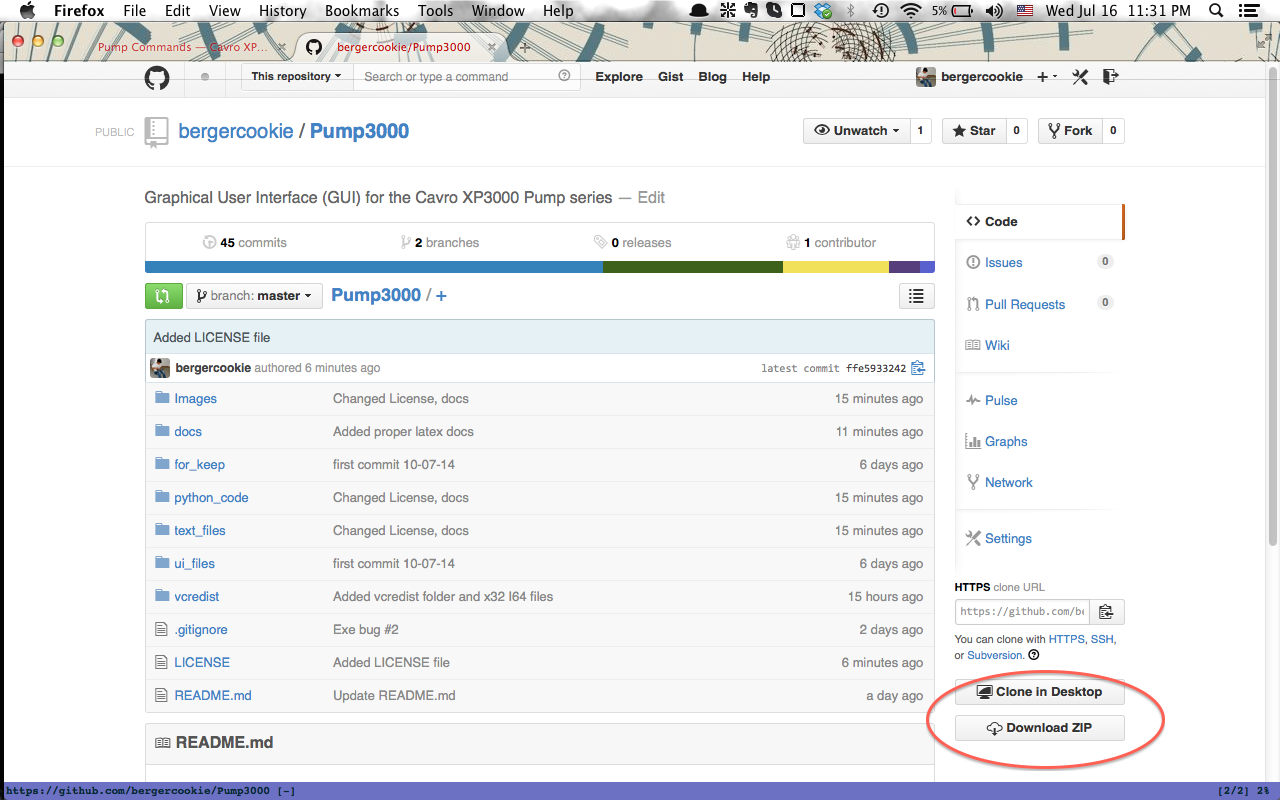
\includegraphics{downloading.png}
\caption{Downloading the software}\label{getting-started:downloading}\end{figure}

Alternatively the user can \textbf{clone} the project. In order to do that he must first make sure that git is installed
on the platform. If it isn't then installing it requires issuing:

\begin{Verbatim}[commandchars=\\\{\}]
sudo apt\PYGZhy{}get install git \PYGZdq{}for Linux users \PYGZhy{} command\PYGZhy{}line
sudo port install git \PYGZdq{}MacOS users \PYGZhy{} command\PYGZhy{}line
\end{Verbatim}

Then in order to clone the project the user can run the git clone command:

\begin{Verbatim}[commandchars=\\\{\}]
git clone http://wwww.github.com/bergercookie/Cavro\PYGZhy{}Pump\PYGZhy{}XP3000\PYGZhy{}GUI.git
\end{Verbatim}

For windows users, the desktop version of Github is suggested:
\href{https://help.github.com/articles/set-up-git\#platform-windows}{https://help.github.com/articles/set-up-git\#platform-windows}


\section{Hardware Configuration}
\label{hardware:hardware-configuration}\label{hardware::doc}

\subsection{Equipment used}
\label{hardware:equipment-used}\begin{description}
\item[{For the hardware communication to be achieved the following equipment is suggested:}] \leavevmode\begin{itemize}
\item {} 
USB    -\textgreater{}  Serial (RS-232) adapter

\item {} 
RS-232 -\textgreater{}  RS-485 converter

\item {} 
Power cables (Power + GND)

\item {} 
Jumper wires (at least 2 Female to Male)

\item {} 
Breadboard (optional)

\end{itemize}

\end{description}


\subsection{Connecting the XP3000}
\label{hardware:connecting-the-xp3000}
The serial communication with the pump was implemented using the RS-485 serial
protocol.
\begin{figure}[htbp]
\centering
\capstart

\scalebox{0.100000}{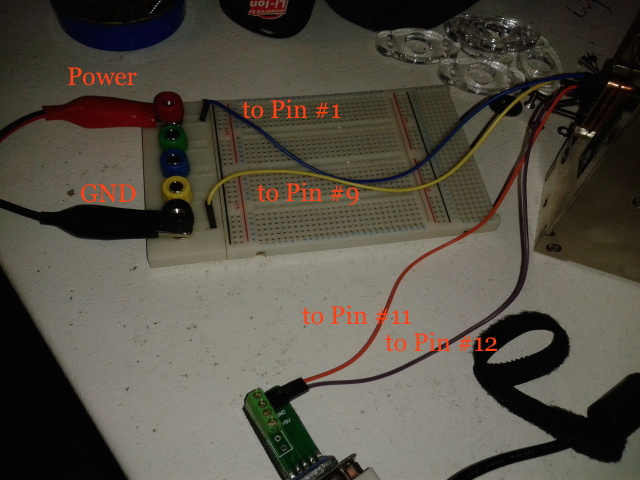
\includegraphics{breadboard.jpg}}
\caption{Suggested Hardware Communication to the pump}\label{hardware:hardware-conf}\end{figure}
\begin{figure}[htbp]
\centering
\capstart

\scalebox{0.100000}{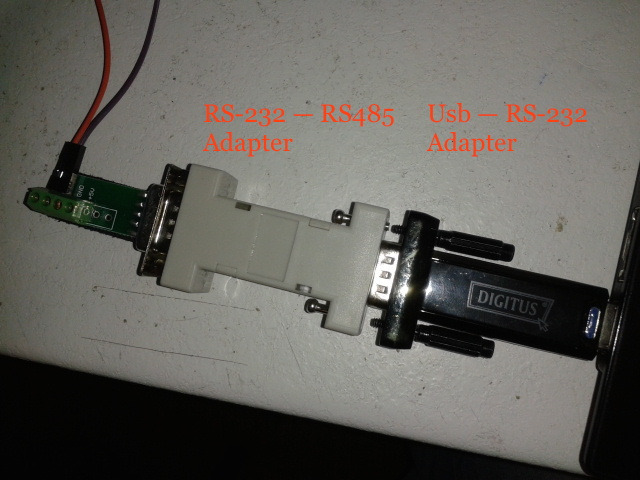
\includegraphics{adapters.jpg}}
\caption{Adapters setup}\label{hardware:adapters}\end{figure}

The needed steps to archive a similar connection would be the following:

1. Connect the pump to a power supply. As described in the
manual the XP3000 requires a \textbf{24VDC power supply} with a current rating of at least \textbf{1.5A}.
As seen in {\hyperref[hardware:hardware-conf]{hardware-conf}}, during the development part, the power was supplied indirectly to the pump
first by running the supply cables into a breadboard and then using extra jumpers to
connect to pump pins \#1 (power) and \#9(GND)

2. For the serial communication, you need to connect the RS-485A, RS-485B signals from the pump PCB
into the RS-485+, RS-485- of the data terminal (PC) used for the communication.
Take extra notice when it comes to connecting the jumpers from the serial adapter
to the pump PCB corresponding pins

3. Also if the computer in use doesn't have a serial port available, the user should use either
a USB to RS-485 adapter, or combine a more commonly found \emph{USB to RS-232 with a RS-232 to
RS-485} {\hyperref[hardware:adapters]{adapters}}

To sum it up, here is the typical RS-485 pinout for the pump \footnote{
For more information regarding the pump pinout consult the pump manual
}, as it is described above

\begin{tabulary}{\linewidth}{|L|L|L|}
\hline
\textsf{\relax 
Role
} & \textsf{\relax 
Pin No
} & \textsf{\relax 
Signal to Connect
}\\
\hline \multirow{2}{*}{
\textbf{Power}
} & 
\#1 {[}Power{]}
 & 
24 VDC
\\
 & 
\#9 {[}GND{]}
 & 
Ground (of the power supply)
\\
 \multirow{2}{*}{
\textbf{Protocol}
\textbf{Signals}
} & 
\#11 {[}RS-485A{]}
 & 
RS-485 (+)
\\
 & 
\#12 {[}RS-385B{]}
 & 
RS-485 (-)
\\
\hline\end{tabulary}



\section{Software Configuration}
\label{installation:software-configuration}\label{installation::doc}
By now the user should have a copy of the project on his machine. If not refer
to section: {\hyperref[getting-started::doc]{\emph{Getting Started}}}


\subsection{Windows Installation}
\label{installation:running-it}\label{installation:windows-installation}
There are two ways of running the software on windows:
\begin{itemize}
\item {} 
Running the executable

\item {} 
Running from source

\end{itemize}


\subsubsection{Running the executable}
\label{installation:running-the-executable}
\textbf{Running the executable} is as simple as running the Pump3000.exe
located in the \textless{}location\_to\_project\textgreater{}/python\_code/dist folder \footnote{
You can make a shortcut to Pump.exe file but do not move it outside
the dist folder as it depends on the dlls files located there
} \footnote{
If the executable doesn't run correctly, try installing the vcredist\_XXX file.
Replace the XXX with the architecture of your processor.
The vcredist files are located in the vcredist directory.
After the installation, rerun the executable.
If the problem persists, \href{http://www.github.com/bergercookie}{contact me}
}.
\begin{figure}[htbp]
\centering
\capstart

\scalebox{0.100000}{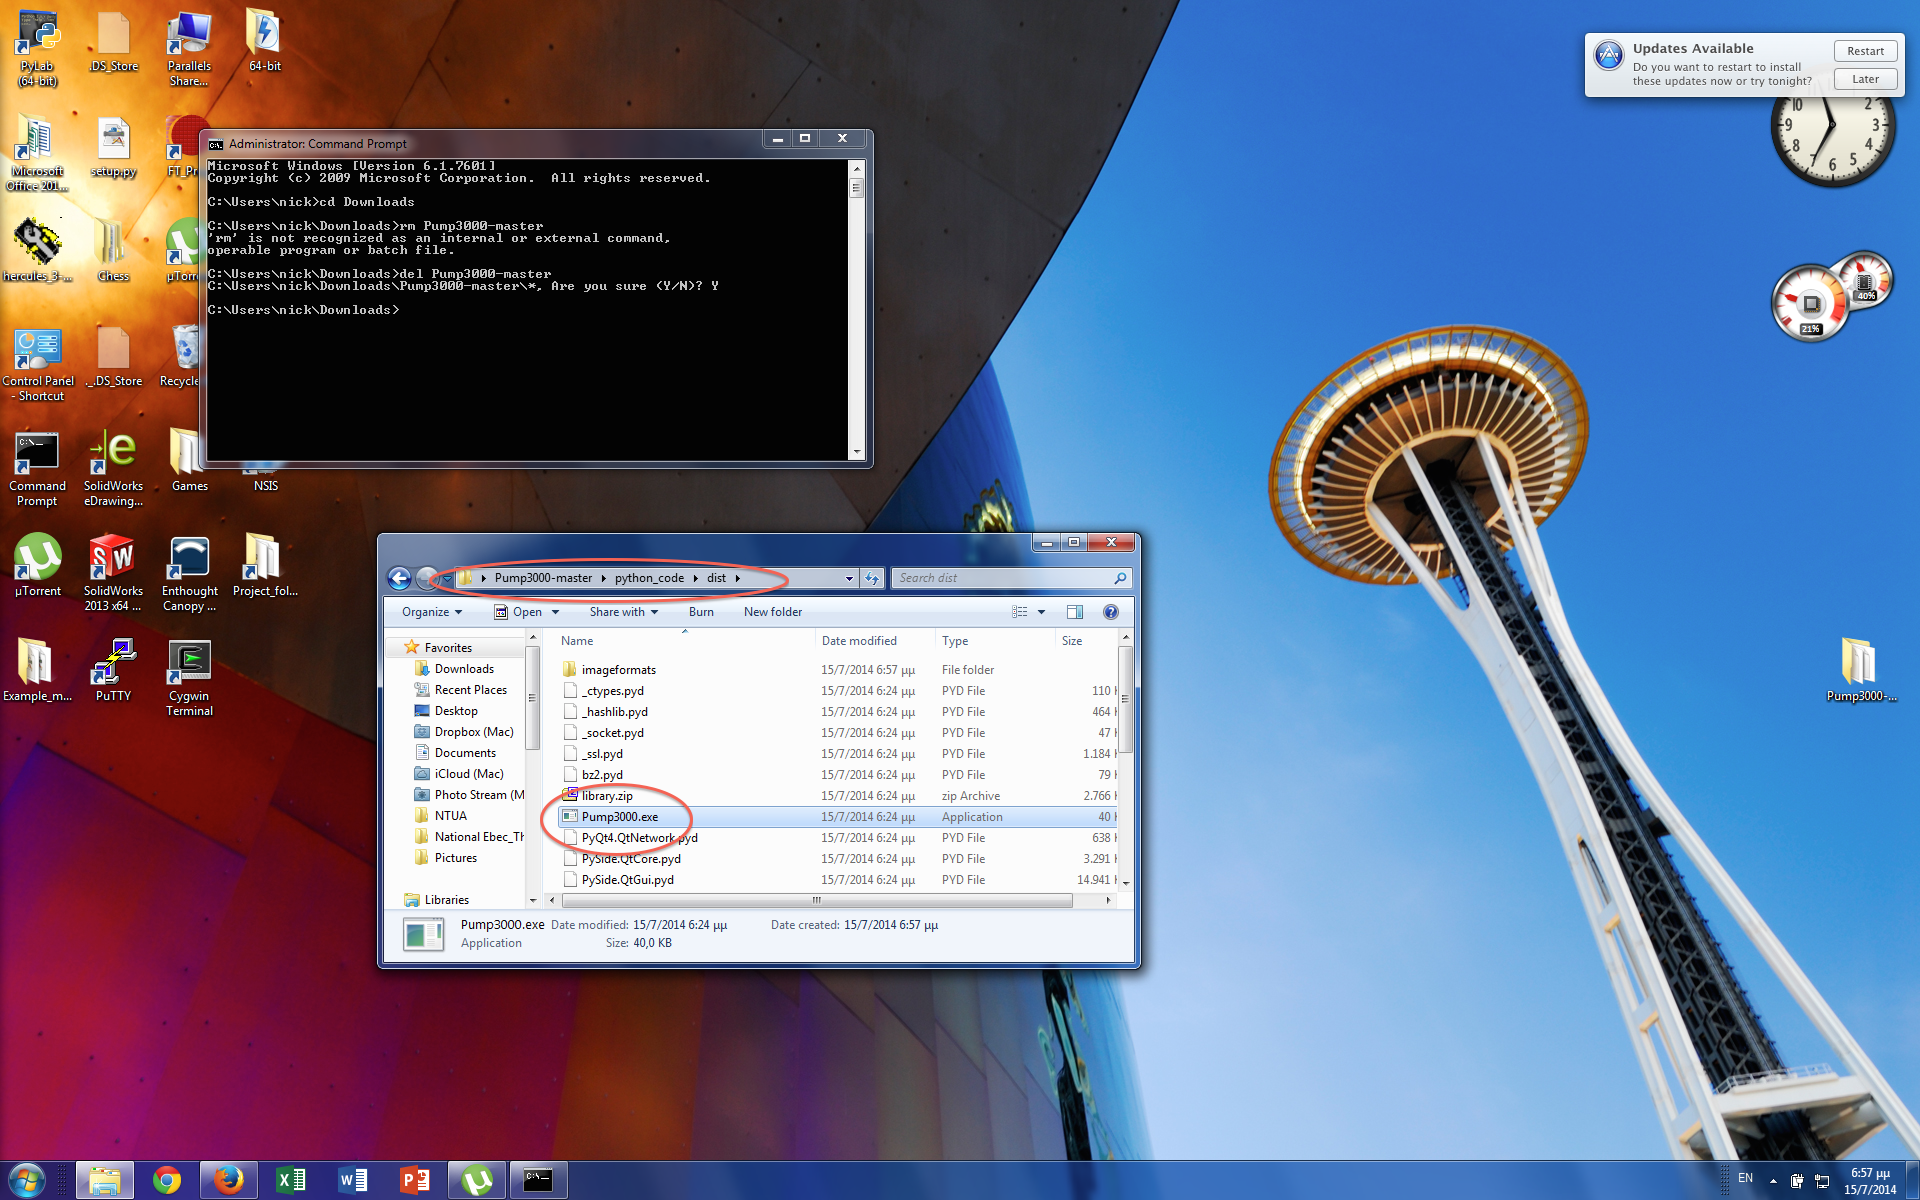
\includegraphics{finding-exe.png}}
\caption{Finding the .exe file}\end{figure}


\subsubsection{Running from source}
\label{installation:running-from-source}
Alternatively, the user can \textbf{run the software from source}. This requires the execution
of a full python distribution. It is advised that the user uses one of the following distributions
due to the simplicity of the installation process
\begin{itemize}
\item {} 
\href{http://continuum.io/downloads}{Anaconda}

\item {} 
\href{https://store.enthought.com/downloads/}{Canopy}

\end{itemize}

The user must also have the following packages installed:
\begin{itemize}
\item {} 
\href{http://pyserial.sourceforge.net/}{Pyserial}

\item {} 
\href{http://qt-project.org/wiki/pyside}{PySide}

\end{itemize}

For the Anaconda distribution the user can install packages from the Command line
using one of the following ways \footnote{
Consult the instructions on the site of the corresponding distribution for more details on
installing packages
}

\begin{Verbatim}[commandchars=\\\{\}]
\PYGZdl{}conda install \PYGZlt{}package\PYGZus{}name\PYGZgt{}

\PYGZdl{}pip install \PYGZlt{}package\PYGZus{}name\PYGZgt{}
\end{Verbatim}

Finally, the user should run the software using the command prompt:

\begin{Verbatim}[commandchars=\\\{\}]
python \PYGZlt{}location\PYGZus{}to\PYGZus{}project\PYGZgt{}\PYGZbs{}python\PYGZus{}code\PYGZbs{}Pump3000.py
\end{Verbatim}


\subsection{Linux/Mac Installation}
\label{installation:linux-mac-installation}
In case the user wants to run the software from a *NIX environment, a basic python distribution
must be installed on the platform, (already preconfigured on most *NIX systems).
The user must also have the following packages installed:
\begin{itemize}
\item {} 
\href{http://pyserial.sourceforge.net/}{Pyserial}

\item {} 
\href{http://qt-project.org/wiki/pyside}{PySide}

\end{itemize}

After this configuration, the user can run the software from the command-line {[}*NIX{]}
command-prompt {[}Windows{]}:

\begin{Verbatim}[commandchars=\\\{\}]
python Pump3000.py
\end{Verbatim}

Note that the user should first go to the folder, the Pump3000.py is located.
\begin{figure}[htbp]
\centering
\capstart

\scalebox{0.100000}{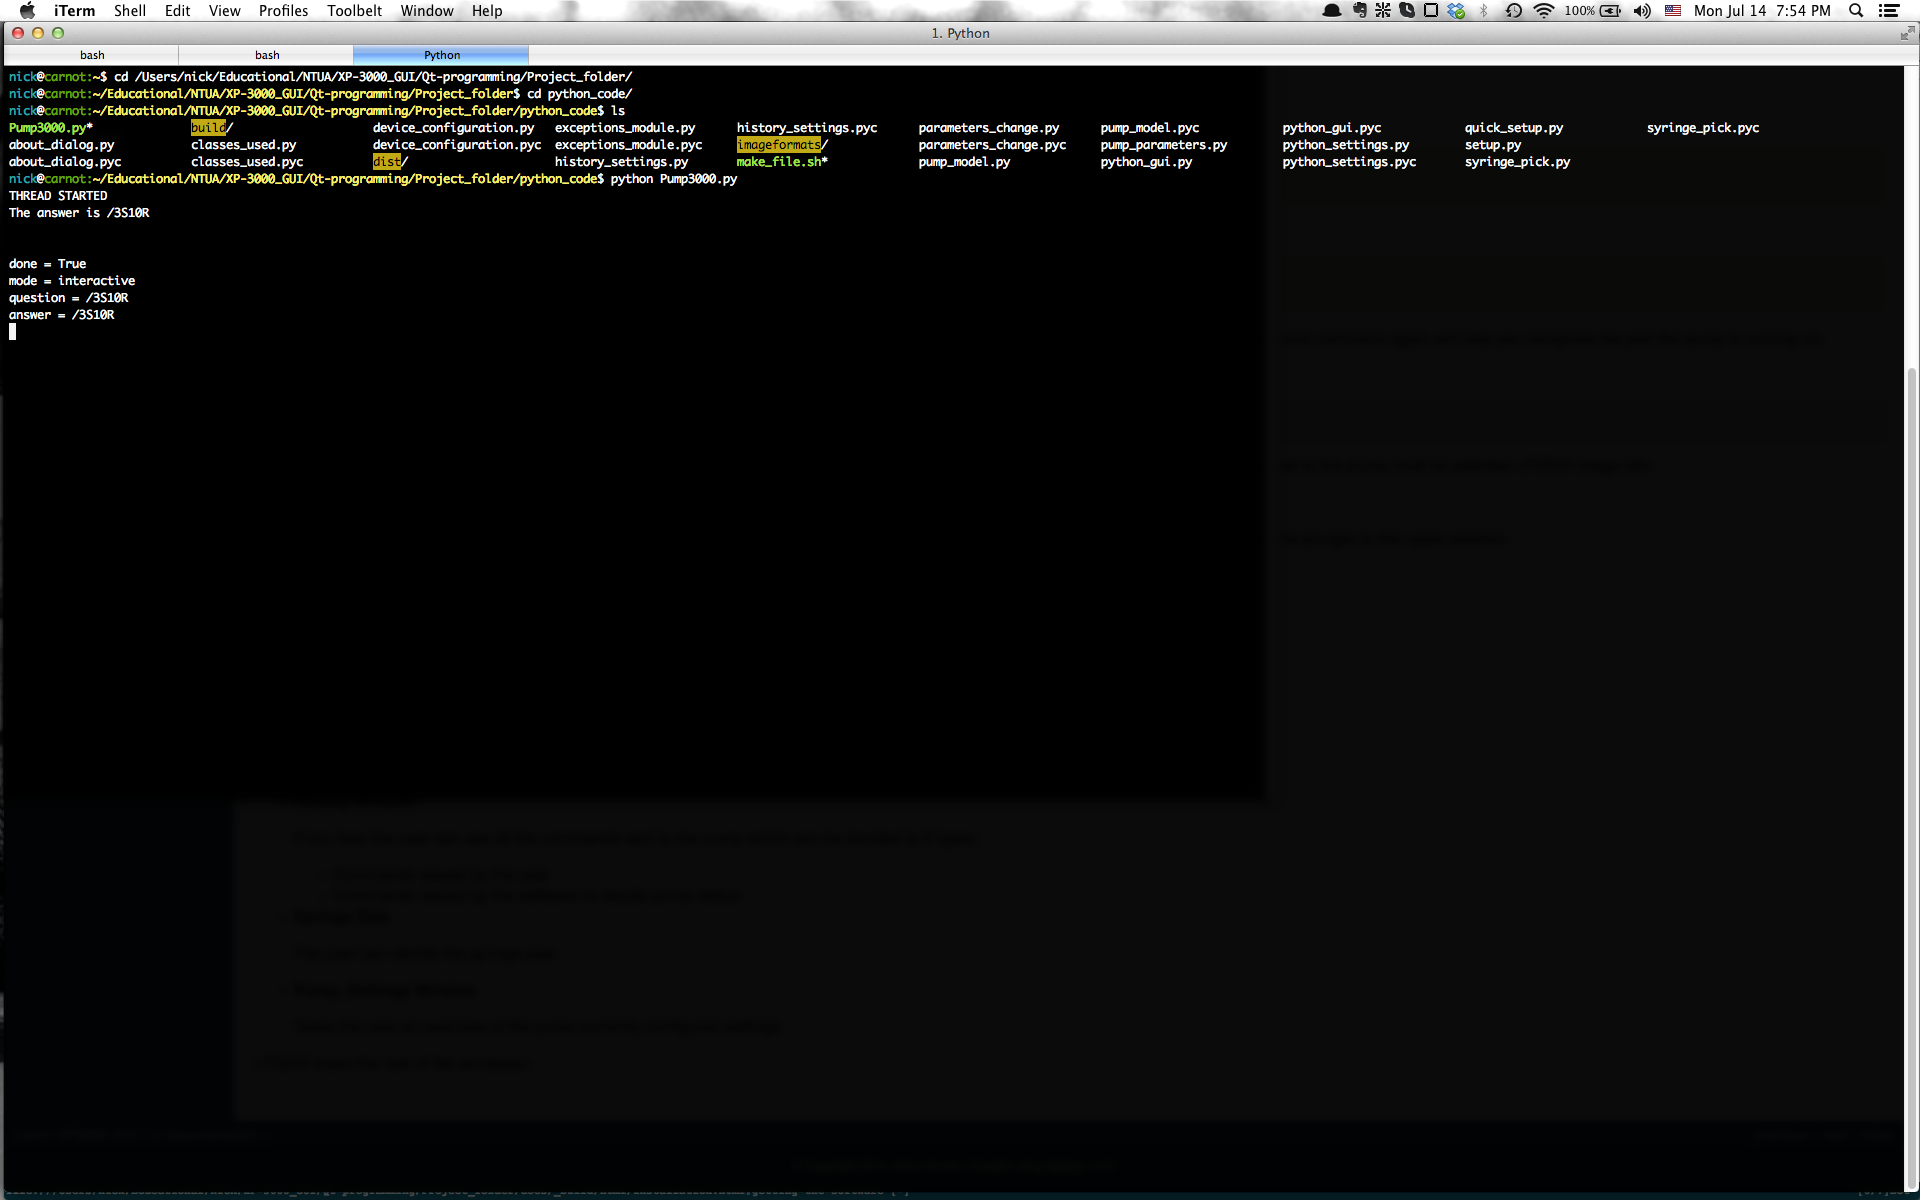
\includegraphics{running-py.png}}
\caption{Running from source on MacOS}\end{figure}


\subsection{Using the software}
\label{installation:using-the-software}
The first thing the user should do, if he doesn't know the serial connector
to the pump, is figure out the correct port:
\begin{itemize}
\item {} 
On \textbf{Windows} machines this can be done by getting the \emph{`Ports (COM \& LPT)'} tab:

\begin{Verbatim}[commandchars=\\\{\}]
Start Menu \PYGZgt{} right\PYGZhy{}click \PYGZdq{}My Computer\PYGZdq{} \PYGZgt{} select \PYGZdq{}Manage\PYGZdq{} \PYGZgt{}  Click on the \PYGZdq{}Device Manager\PYGZdq{}

(On the \PYGZdq{}Device Manager\PYGZdq{}) Click \PYGZdq{}Ports (COM \PYGZam{} LPT)\PYGZdq{} tab \PYGZgt{} select the port your connector is on
\end{Verbatim}

See {\hyperref[installation:finding-manage]{\emph{`Manage' tab}}}, {\hyperref[installation:finding-com-ports]{\emph{Configuring COM ports}}}

\item {} 
On \textbf{*NIX} machines this can be done the following way:

\begin{Verbatim}[commandchars=\\\{\}]
cd /dev

ls \PYGZhy{}lart\textbar{} grep tty
\end{Verbatim}

\end{itemize}

This will give  you a list of the currently available ports. Ejecting and reinserting the connector
to the computer and in the meantime running the second command again will help you recognise
the port the pump is running on.
\begin{figure}[htbp]
\centering
\capstart

\scalebox{0.100000}{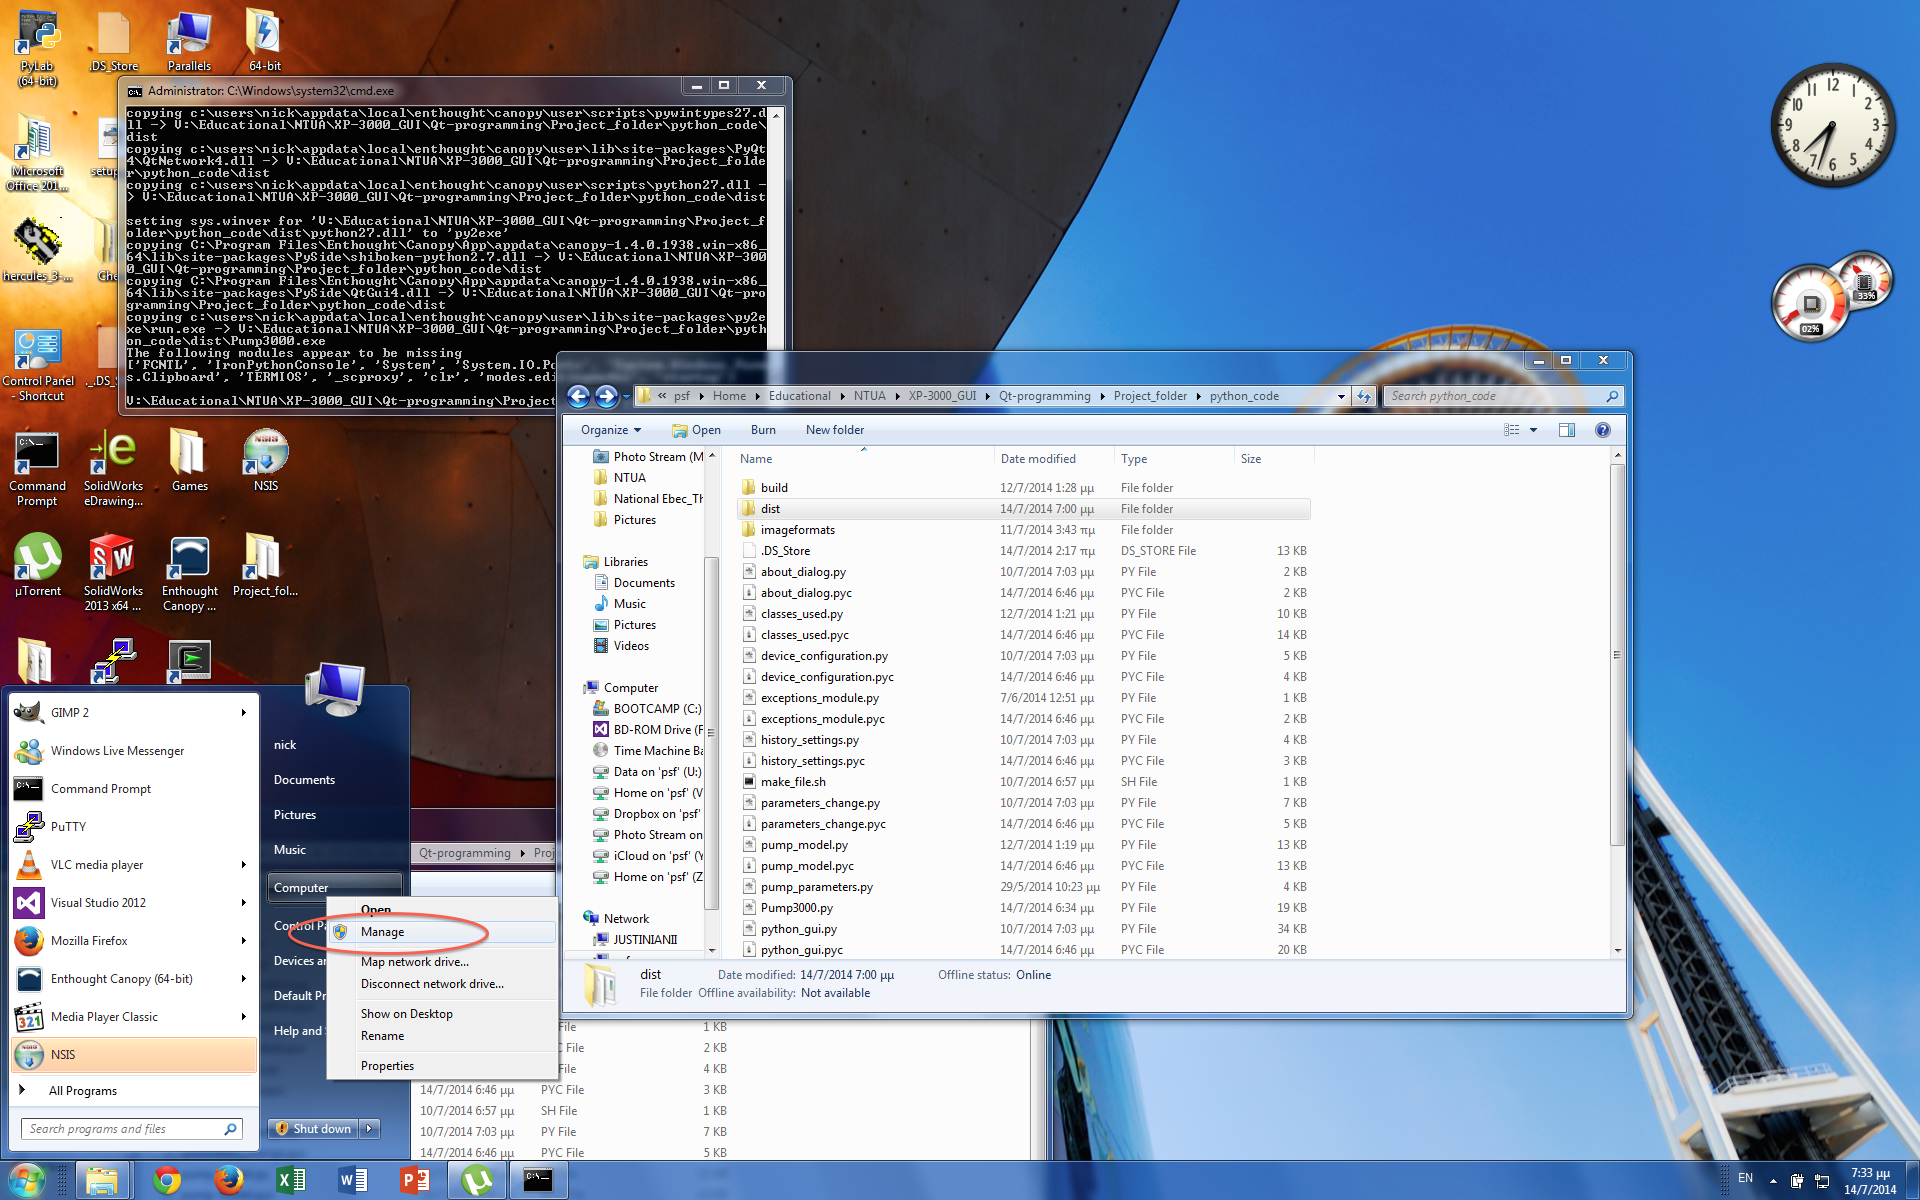
\includegraphics{finding-manage.png}}
\caption{`Manage' tab}\label{installation:finding-manage}\end{figure}
\begin{figure}[htbp]
\centering
\capstart

\scalebox{0.100000}{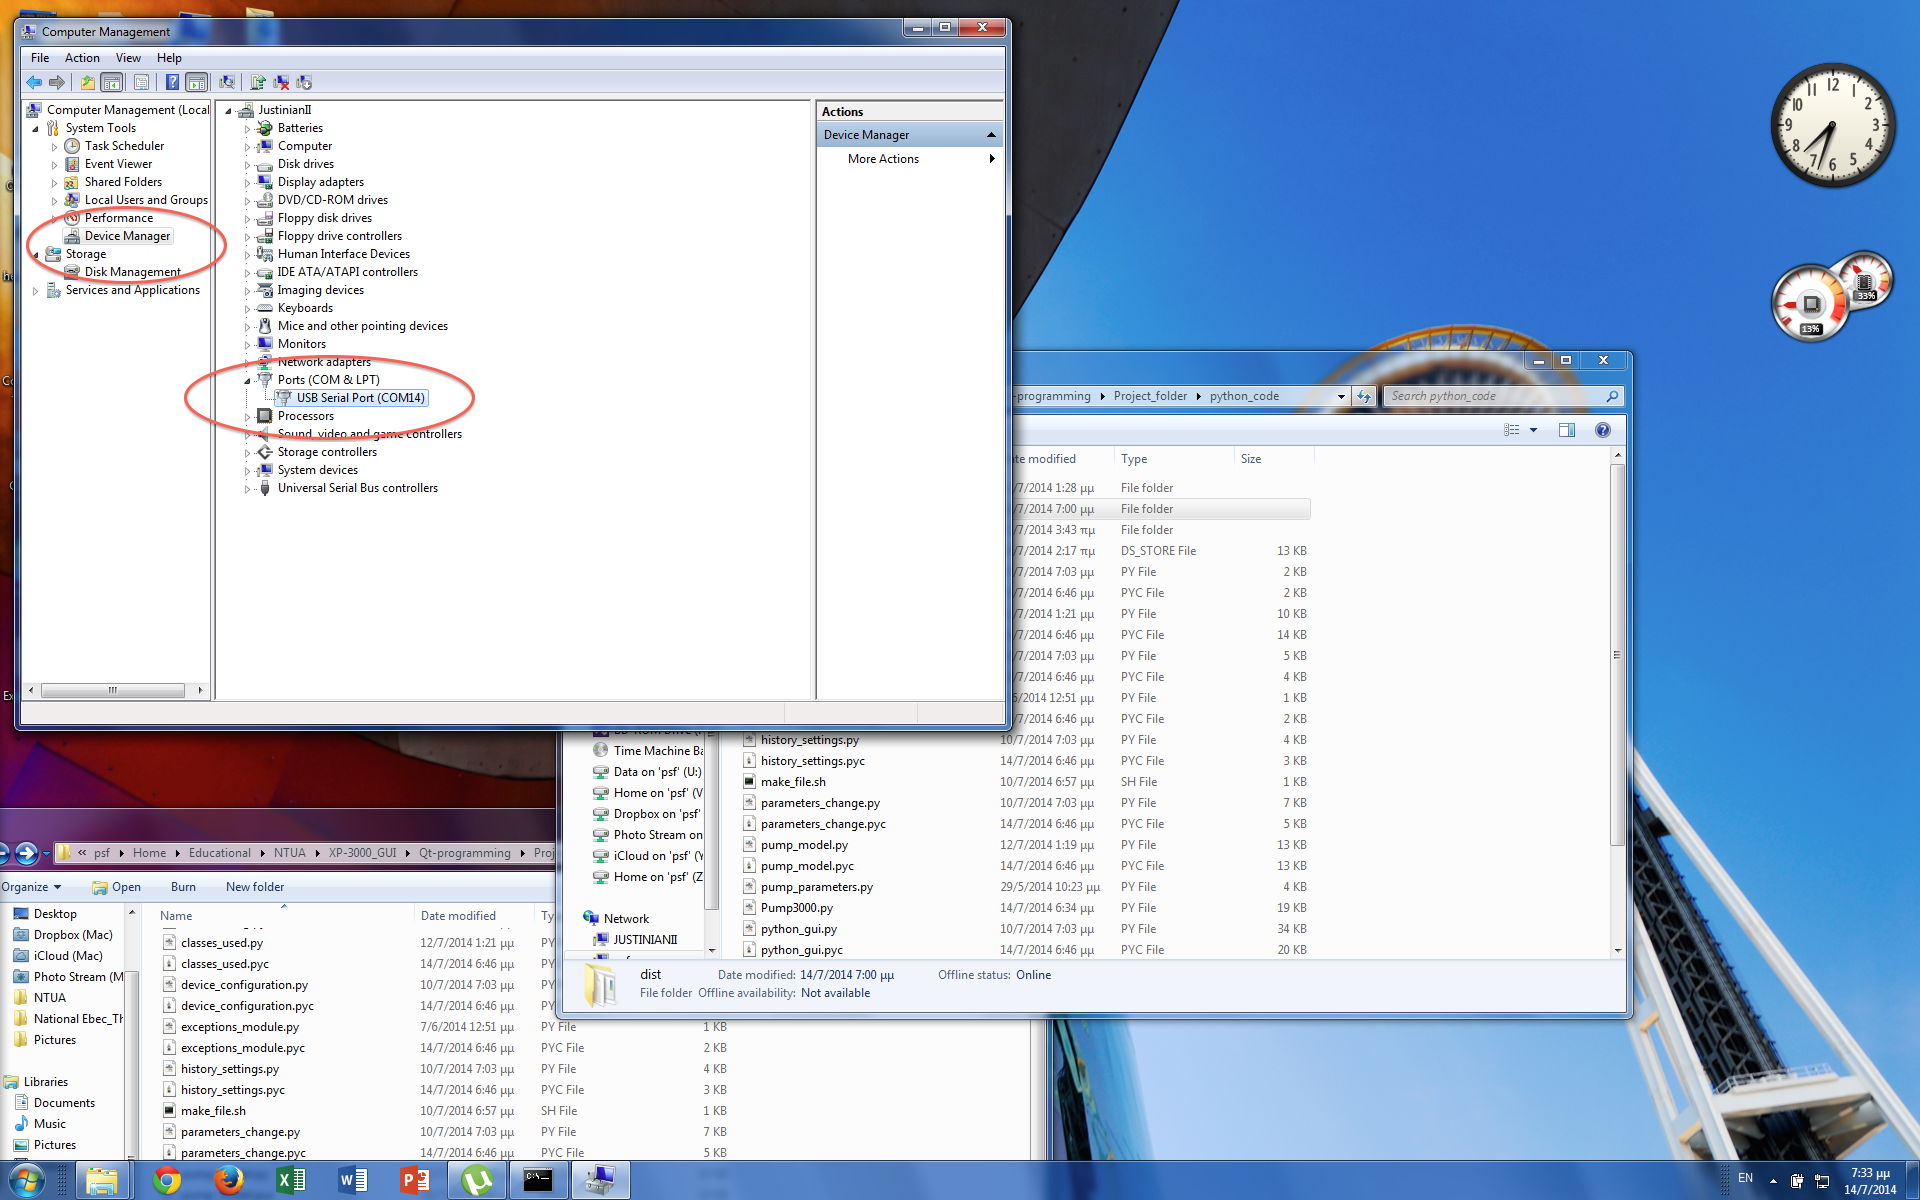
\includegraphics{finding-com-ports.png}}
\caption{Configuring COM ports}\label{installation:finding-com-ports}\end{figure}

\begin{notice}{warning}{Warning:}
Make sure that you have selected the correct port, otherwise the pump will not respond and will
not raise any error Message
\end{notice}

After that you are ready to {\hyperref[installation:running-it]{\emph{run the software}}} (whichever way you want). You should be directed to the New\_Device window where the
port connected to the pump must be selected
\begin{figure}[htbp]
\centering
\capstart

\scalebox{0.100000}{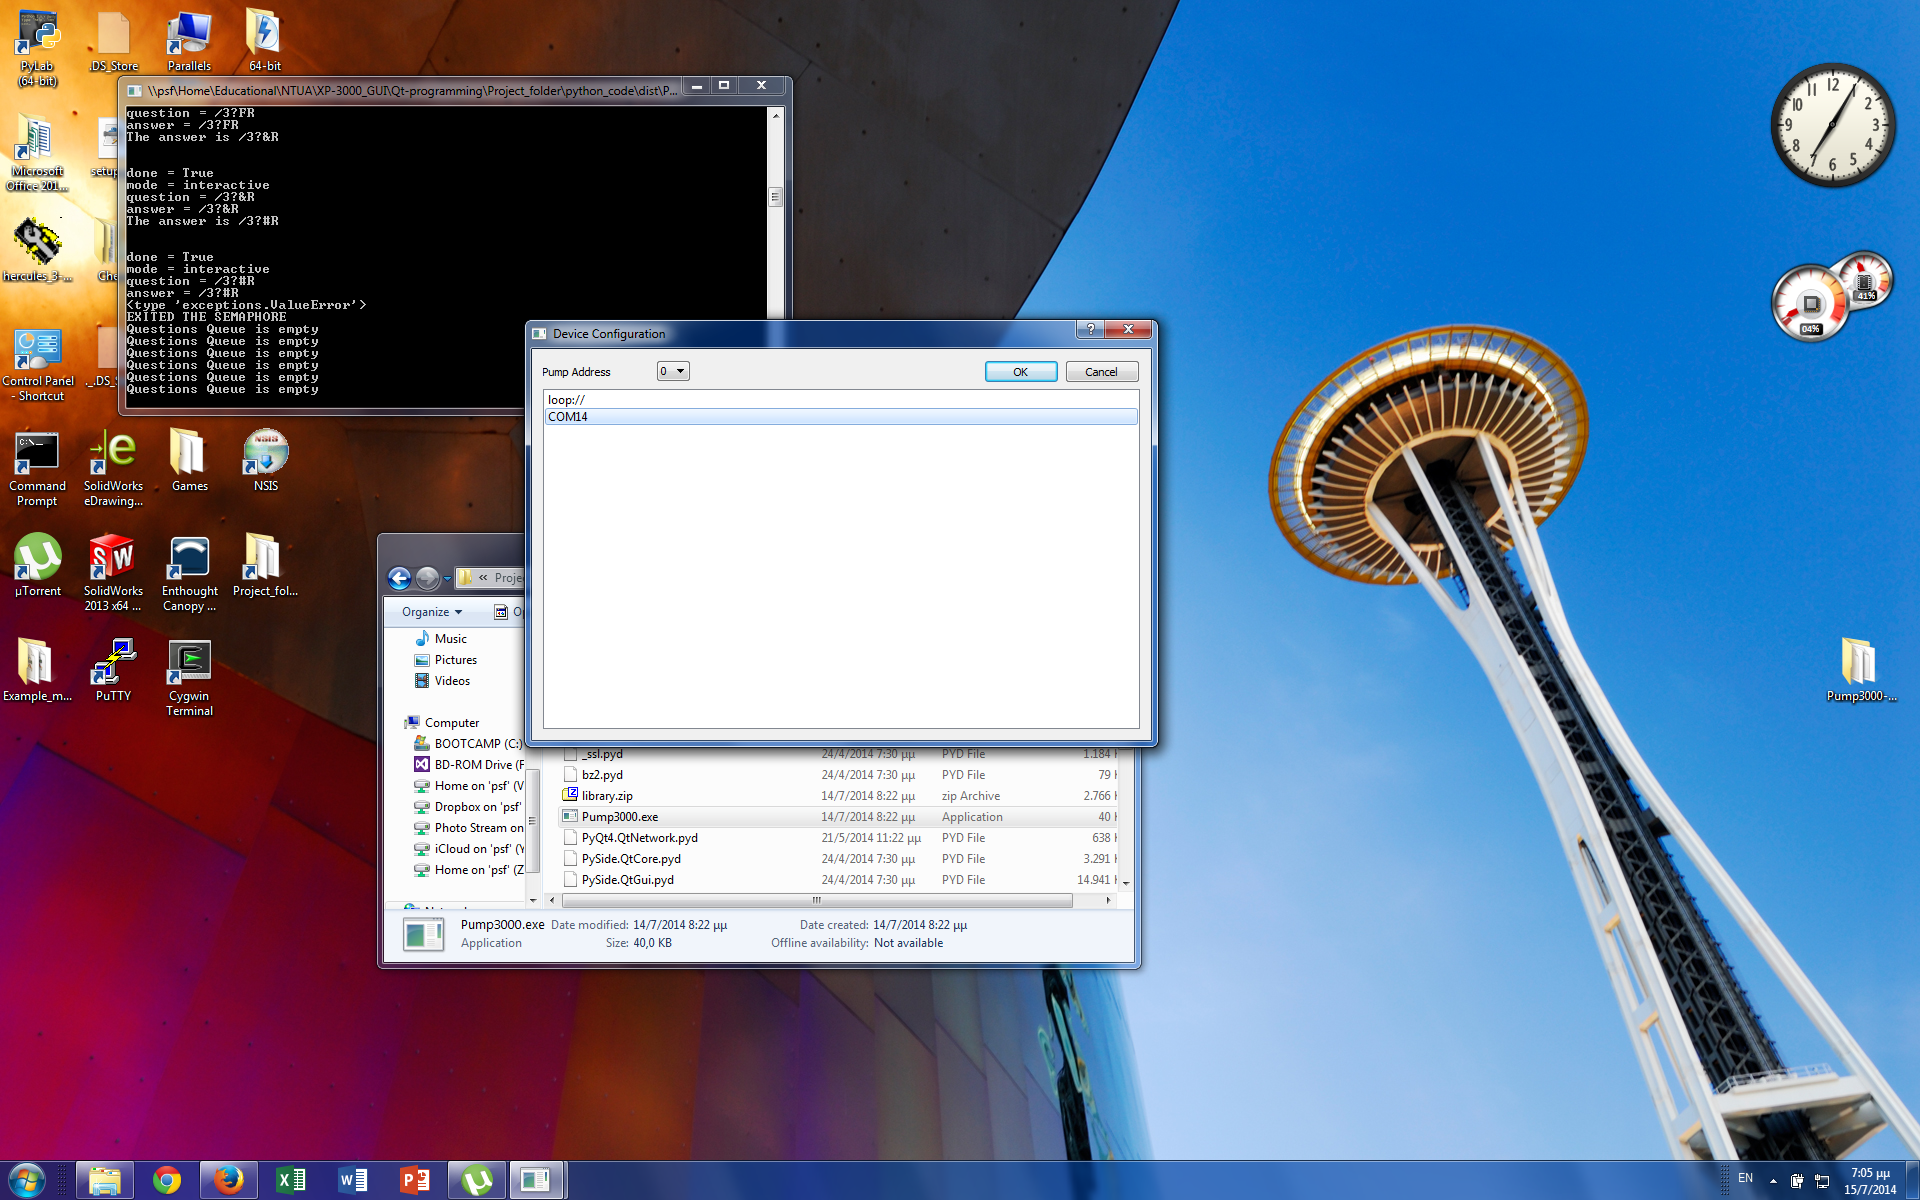
\includegraphics{dev-conf.png}}
\caption{Configuring correct port for pump}\end{figure}

If you have selected the correct port, the connection to the pump is established and
the software will automatically initialize the pump, by moving the plunger to the upper position.

You are now in the Main Window. From here you can:
\begin{itemize}
\item {} 
Command a volume delivery,

\item {} 
Change the speed of the plunger,

\item {} 
Issue a quick command to the pump (halt, push\_all, etc)

\end{itemize}
\begin{figure}[htbp]
\centering
\capstart

\scalebox{0.100000}{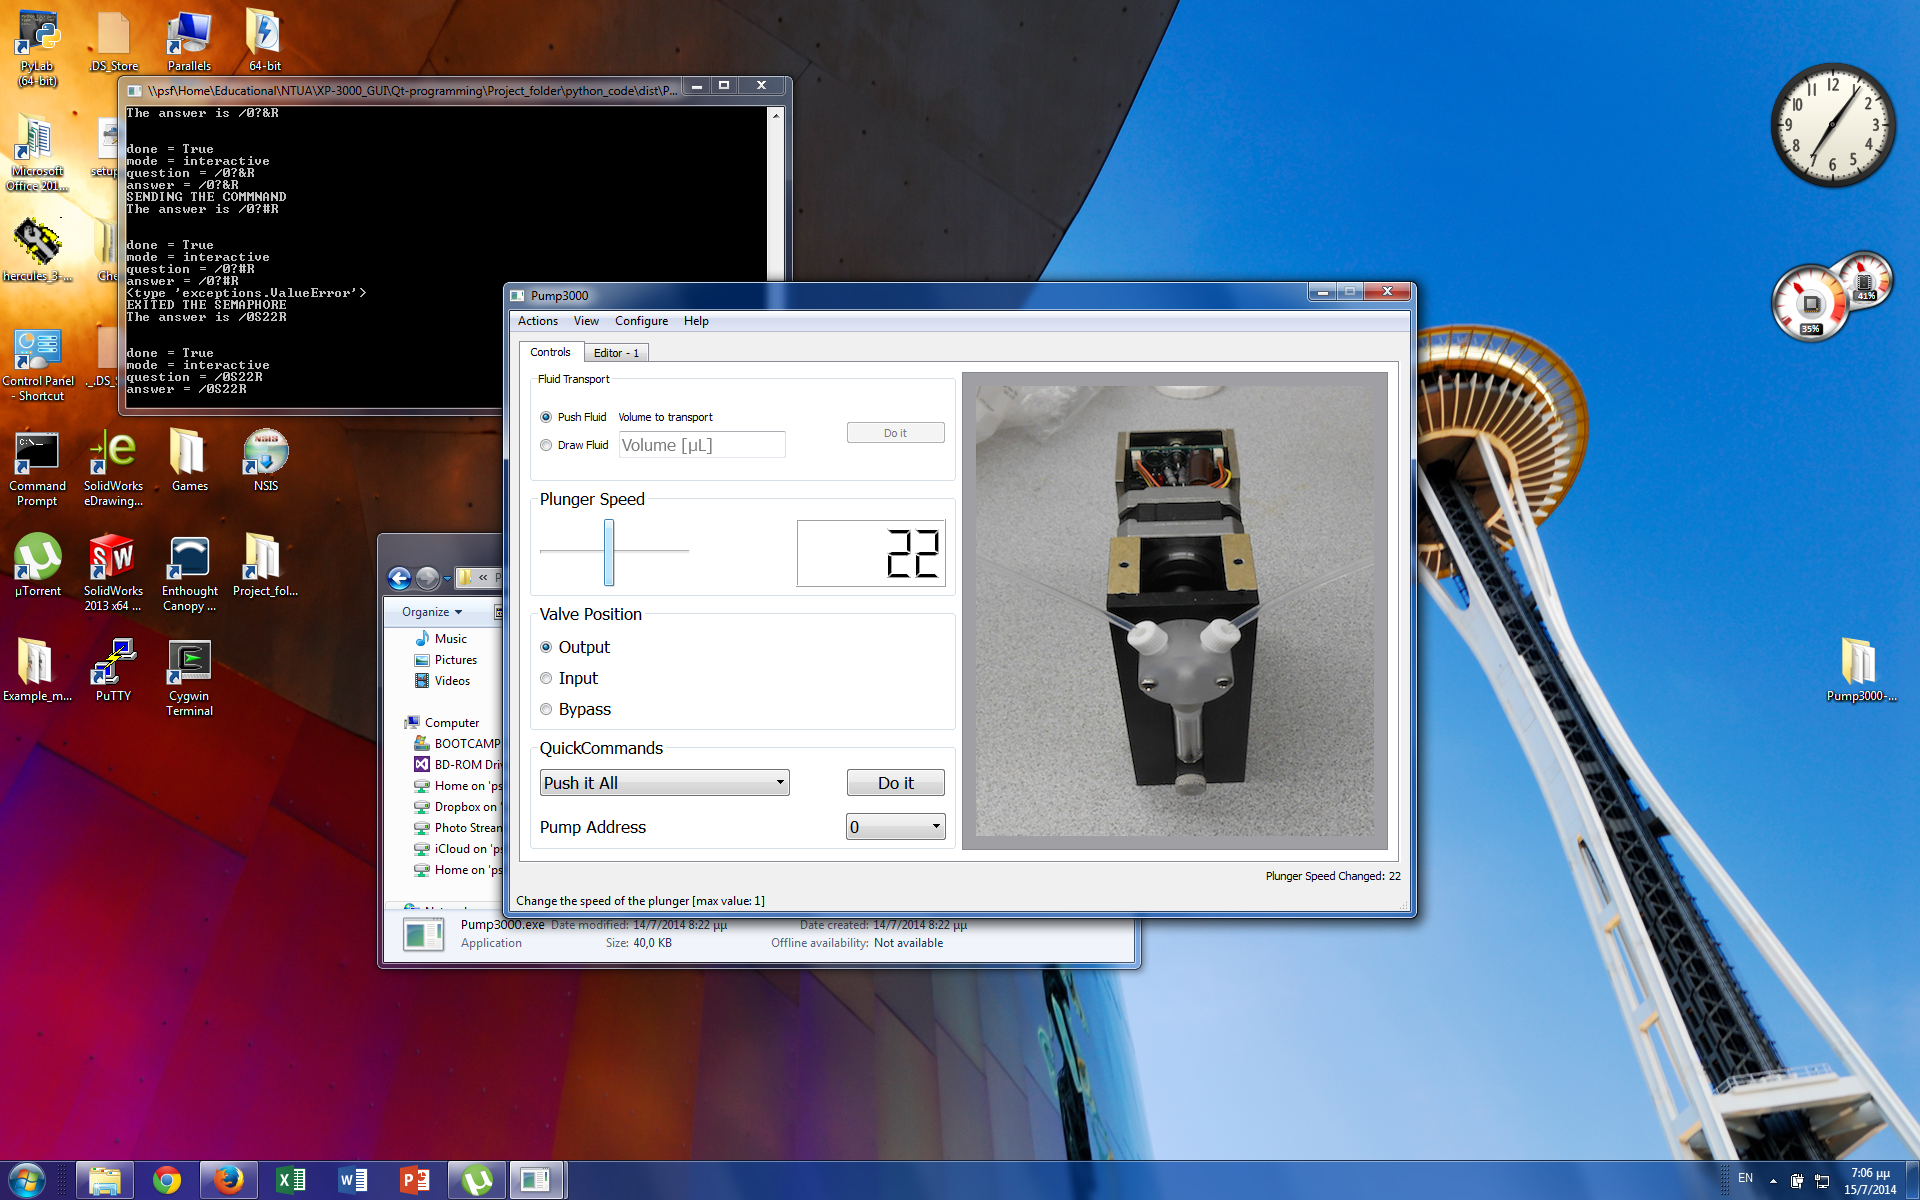
\includegraphics{main-window.png}}
\caption{Main window}\end{figure}

From the main window you can navigate to a series of \textbf{other dialogs:}
\begin{itemize}
\item {} 
\textbf{Editor's Tab}

The Editor's Tab gives the user the ability to issue a series of commands to the pump.
These commands are supplied in the ``Pump Commands'' page. The user can also issue raw
pump commands in the same way.

A typical example of issued commands would be the following:

\begin{Verbatim}[commandchars=\\\{\}]
pump.property\PYGZus{}set(\PYGZsq{}speed\PYGZsq{}, \PYGZsq{}5\PYGZsq{})
\PYGZsh{} Python Comments, write as many as you want
\PYGZsh{} Empty lines don\PYGZsq{}t matter

\PYGZsh{} Raw commands as well
/1?2R\PYGZbs{}r

pump.send\PYGZus{}Command(\PYGZsq{}A0\PYGZsq{})
\end{Verbatim}

\end{itemize}
\begin{figure}[htbp]
\centering
\capstart

\scalebox{0.100000}{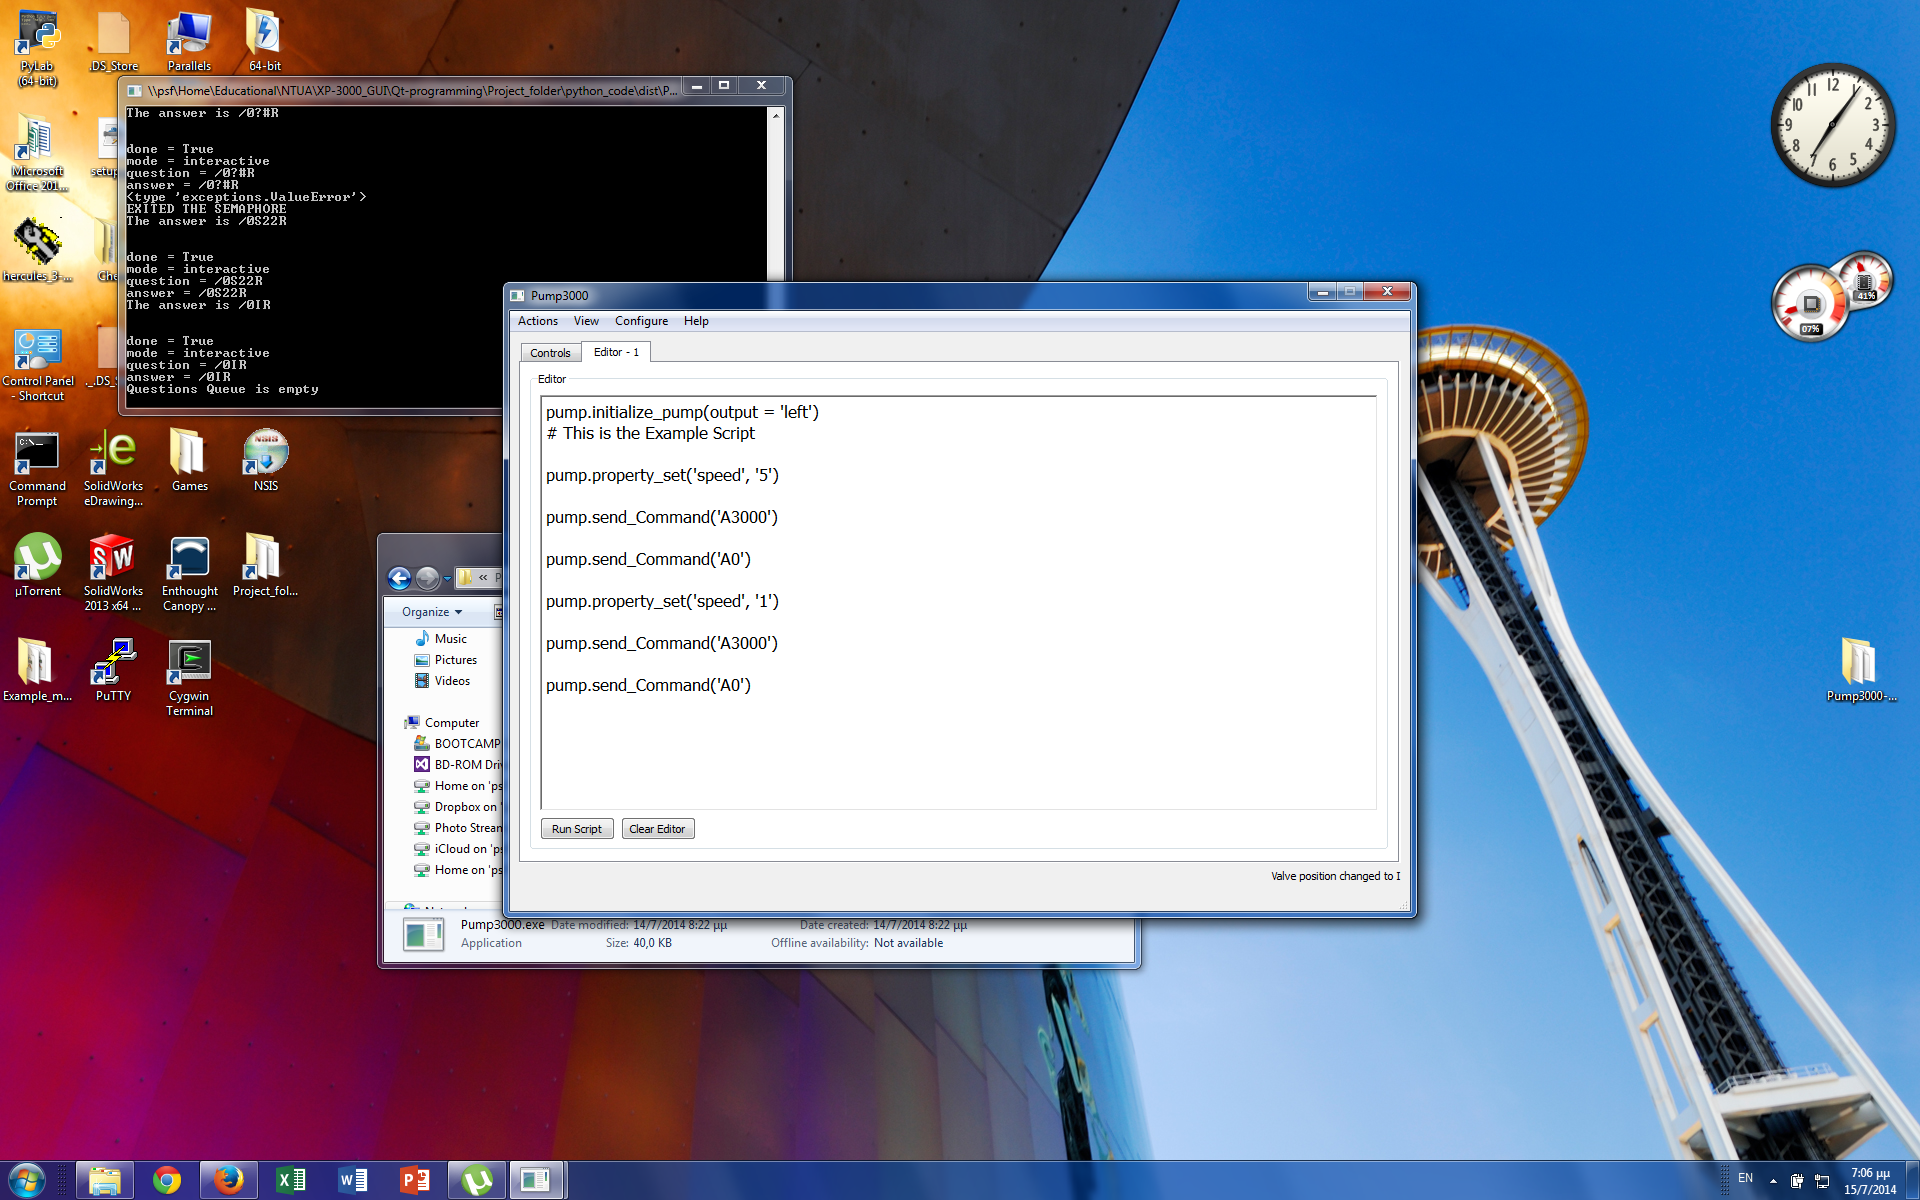
\includegraphics{editor-tab.png}}
\caption{The Editor's Tab}\end{figure}
\begin{itemize}
\item {} 
\textbf{History}

From here the user can see all the commands sent to the pump which can be divided to 2 types:
\begin{itemize}
\item {} 
Commands issued by the user

\item {} 
Commands issued by the software to decide pump status

\end{itemize}

\end{itemize}
\begin{figure}[htbp]
\centering
\capstart

\scalebox{0.100000}{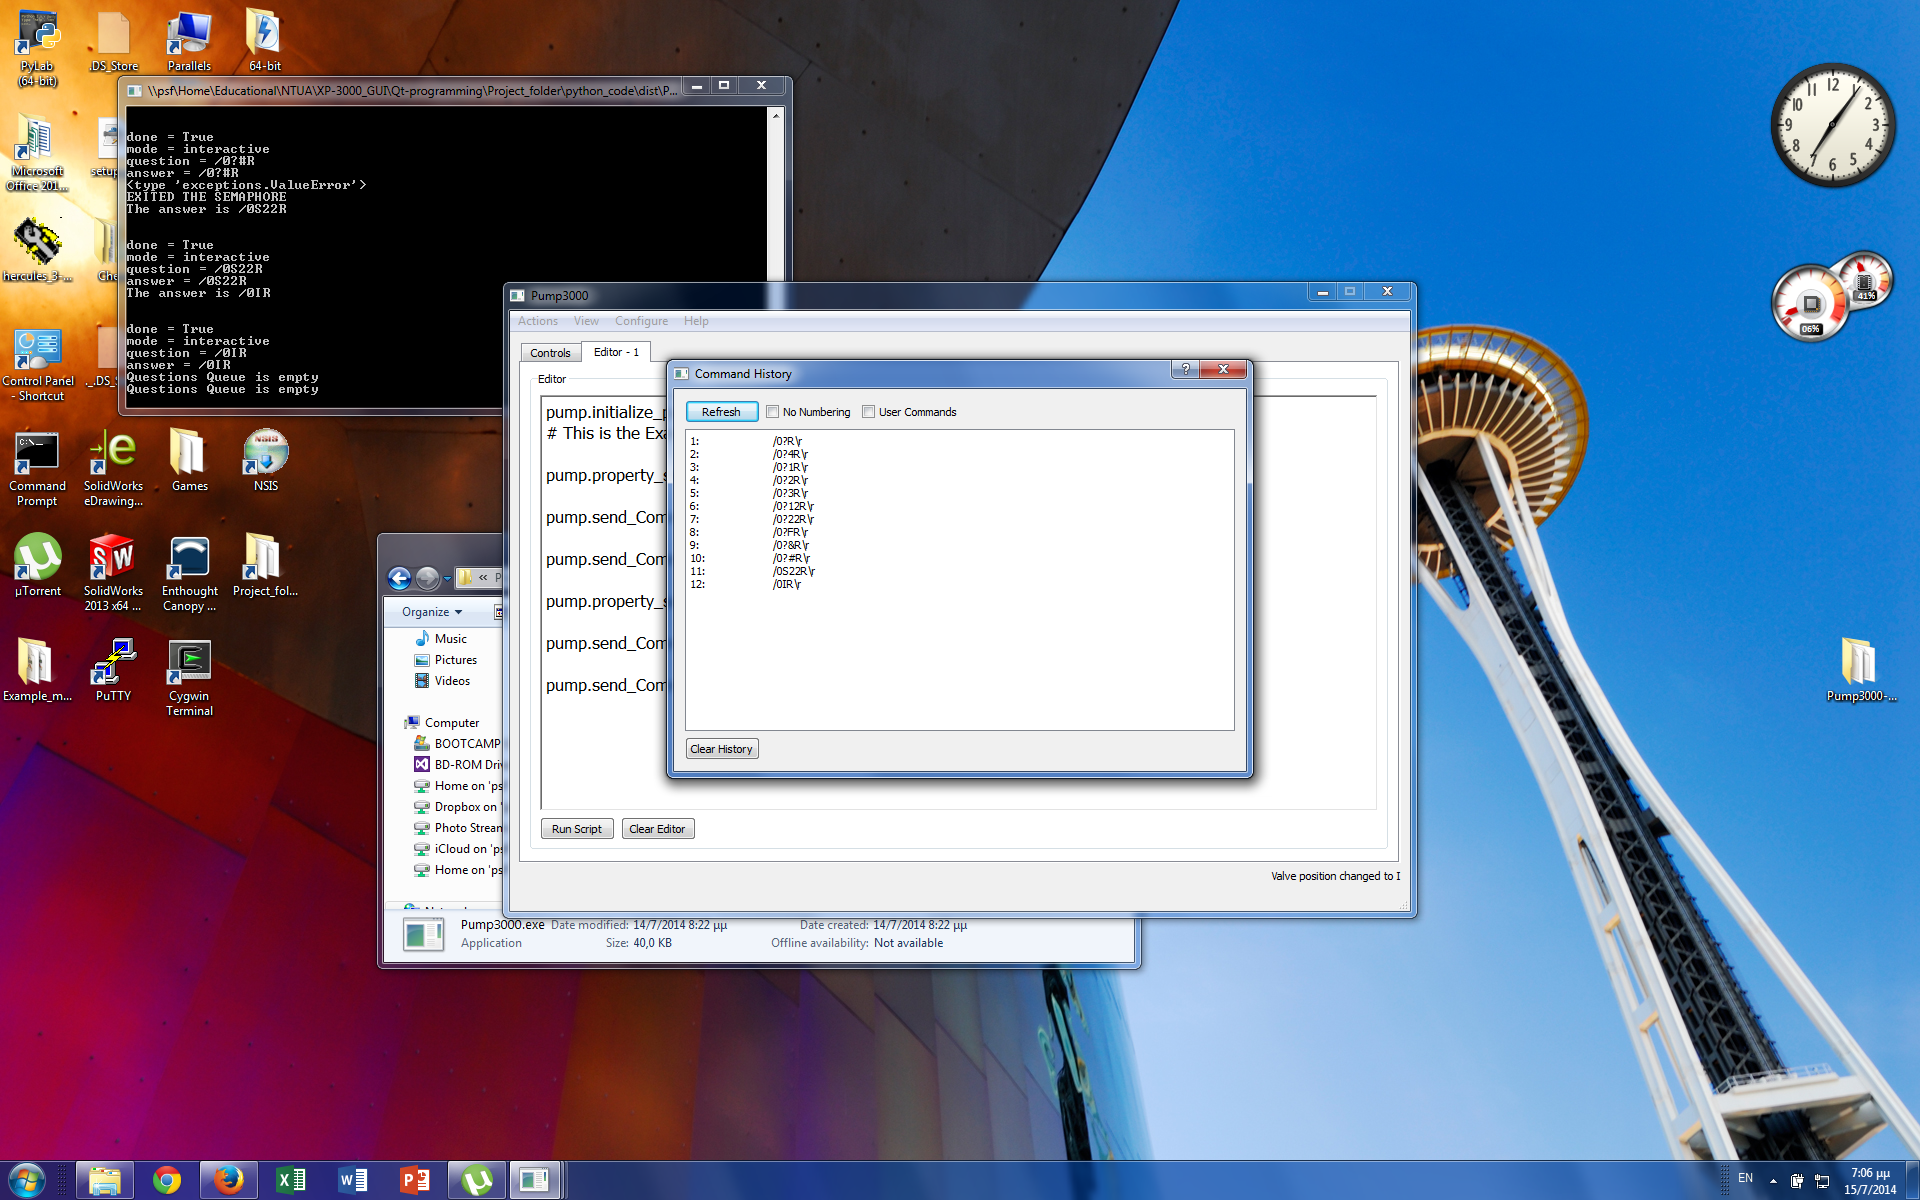
\includegraphics{history-window.png}}
\caption{History window}\end{figure}
\begin{itemize}
\item {} 
\textbf{Syringe Size}

The user can decide the syringe size.

\item {} 
\textbf{Reports}

Gives the user an overview of the pump currently configured settings

\end{itemize}
\begin{figure}[htbp]
\centering
\capstart

\scalebox{0.100000}{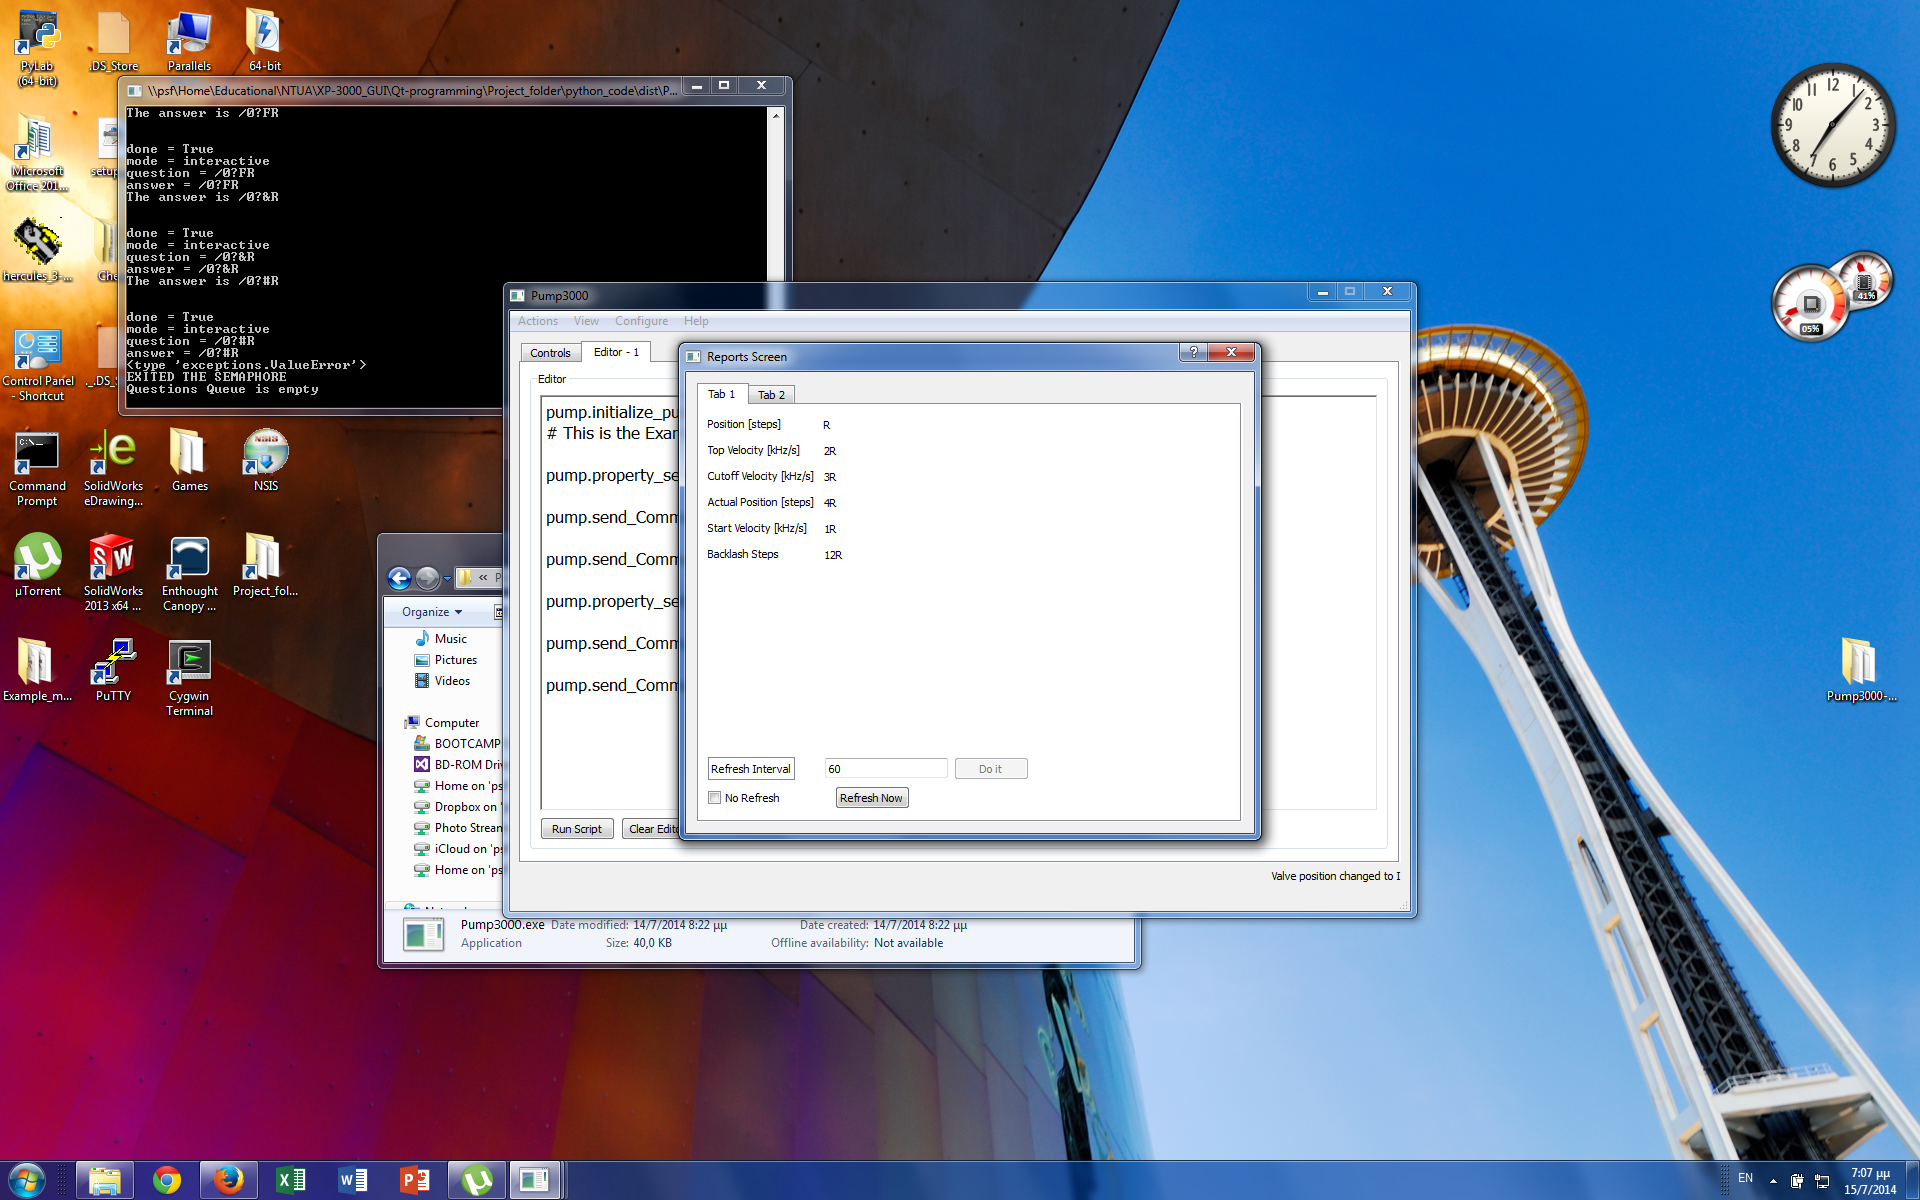
\includegraphics{reports-window.png}}
\caption{Reports window}\end{figure}
\begin{itemize}
\item {} 
\textbf{Pump Parameters}

The user can change certain parameters of the plunger movement such as ``Top Velocity'', ``Slope'' etc.

\textbf{Port}

The user can configure the port that the pump is connected to. This window is
also summoned at the start of the Pump30000

\end{itemize}


\section{Pump Commands}
\label{pump-commands:pump-commands}\label{pump-commands::doc}
In this section the basic commands for communication with the pump are introduced.
You can issue a series of these commands from the editor's tab.
For the full list of available commands see the pump\_model.py. You can use most
of the methods of the Pump Class in the Editor tab as well.

\begin{notice}{note}{Note:}
`self' is a Python class arguement and shouldn't be issued by the user.
\end{notice}

\textbf{pump.connect\_new(self, port\_name)}

\emph{Arguements}:

\begin{Verbatim}[commandchars=\\\{\}]
port\PYGZus{}name: string
\end{Verbatim}

\emph{Description}
\begin{quote}

Connect to the given port address.
\end{quote}

\emph{Example}:

\begin{Verbatim}[commandchars=\\\{\}]
pump.connect\PYGZus{}new({}`/dev/tty.\PYGZhy{}SerialPort1\PYGZhy{}1\PYGZsq{}) \PYGZhy{}\PYGZgt{} Configuring a serial connection on OSX
\end{Verbatim}

\textbf{pump.initialize\_pump(self, output = `right')}

\emph{Arguements}:

\begin{Verbatim}[commandchars=\\\{\}]
output: string [Optional]

    values: \PYGZsq{}left\PYGZsq{}, \PYGZsq{}right\PYGZsq{}
\end{Verbatim}

\emph{Description}
\begin{quote}

Initialize the pump. The user can optionally issue the output valve. By default if not
given otherwise, the output valve is set to the right.
\end{quote}

\emph{Examples}:

\begin{Verbatim}[commandchars=\\\{\}]
pump.initialize\PYGZus{}pump() \PYGZhy{}\PYGZgt{} Initializing the pump with default output valve (right)
pump.initialize\PYGZus{}pump(output = {}`left\PYGZsq{}) \PYGZhy{}\PYGZgt{} Initializing the pump with output valve set to left
\end{Verbatim}

\textbf{pump.valve\_command(self, position)}

\emph{Arguements}:

\begin{Verbatim}[commandchars=\\\{\}]
position: string

    values: \PYGZsq{}I\PYGZsq{} (Input)
            \PYGZsq{}O\PYGZsq{} (Output)
            \PYGZsq{}B\PYGZsq{} (Bypass)
\end{Verbatim}

\emph{Description}
\begin{quote}

Set the valve to certain position.
\end{quote}

\emph{Examples}:

\begin{Verbatim}[commandchars=\\\{\}]
pump.valve\PYGZus{}command({}`B\PYGZsq{}) \PYGZhy{}\PYGZgt{} Set the valve to Bypass position
\end{Verbatim}

\textbf{pump.property\_set(self, a\_proprty, value)}

\emph{Arguements}:

\begin{Verbatim}[commandchars=\\\{\}]
a\PYGZus{}property : string
value      : int
\end{Verbatim}

\emph{Description}
\begin{quote}

Set a certain property for the plunger. The following properties are available for
modification. These are listed with regards to the command that should be issued
and the range of the values permitted:

\begin{Verbatim}[commandchars=\\\{\}]
\PYGZsq{}speed\PYGZsq{}                 : \PYGZsq{}S\PYGZsq{}, [1  , 40]
\PYGZsq{}backlash\PYGZsq{}              : \PYGZsq{}K\PYGZsq{}, [0  , 31]
\PYGZsq{}slope                  : \PYGZsq{}L\PYGZsq{}, [1  , 20]
\PYGZsq{}start\PYGZus{}velocity\PYGZsq{}        : \PYGZsq{}v\PYGZsq{}, [50 , 1000]
\PYGZsq{}top\PYGZus{}velocity\PYGZsq{}          : \PYGZsq{}V\PYGZsq{}, [5  , 5800]
\PYGZsq{}cutoff\PYGZus{}velocity\PYGZsq{}       : \PYGZsq{}c\PYGZsq{}, [50 , 2700]
\PYGZsq{}cuttof\PYGZus{}velocity\PYGZus{}steps\PYGZsq{} : \PYGZsq{}C\PYGZsq{}, [0  , 25]
\end{Verbatim}

The user is encouraged to consult the manual for an overview on the
commands above
\end{quote}

\emph{Examples}:

\begin{Verbatim}[commandchars=\\\{\}]
pump.property\PYGZus{}set({}`speed\PYGZsq{}, {}`10\PYGZsq{}) \PYGZhy{}\PYGZgt{} Set the plunger speed to 10
pump.property\PYGZus{}set({}`backlash\PYGZsq{}, {}`15\PYGZsq{}) \PYGZhy{}\PYGZgt{} set the backlash steps to 15
\end{Verbatim}

\textbf{pump.volume\_command(self, direction = {}`P', vol = {}`0', special=None)}

\emph{Arguements}:

\begin{Verbatim}[commandchars=\\\{\}]
direction : string

    Values: \PYGZsq{}P\PYGZsq{}
            \PYGZsq{}D\PYGZsq{}

vol       : string [Microliters]

special   : string [Optional]

    Values: \PYGZsq{}push\PYGZus{}all\PYGZsq{}
            \PYGZsq{}pull\PYGZus{}all\PYGZsq{}
\end{Verbatim}

\emph{Description}
\begin{quote}

Volume pushing / drawing mechanism. The user can issue a volume delivery as well
as issue a special push / pull all action. In case the special action is given,
the  `vol' argument is neglected
\end{quote}

\emph{Examples}:

\begin{Verbatim}[commandchars=\\\{\}]
pump.volume\PYGZus{}command(direction = \PYGZsq{}D\PYGZsq{}, vol = \PYGZsq{}5\PYGZsq{}) \PYGZhy{}\PYGZgt{} Dispense 5 microlitres
pump.volume\PYGZus{}command(special = {}`push\PYGZus{}all\PYGZsq{}) \PYGZhy{}\PYGZgt{} Dispense fluid volume
\end{Verbatim}

\textbf{pump.send\_Command(self, command, bits\_on\_return = 0)}

\emph{Arguements}:

\begin{Verbatim}[commandchars=\\\{\}]
command        : string
bits\PYGZus{}on\PYGZus{}return : int [Optional]
\end{Verbatim}

\emph{Description}
\begin{quote}

Sending Commands to the pump.
Consult the manual for a detailed list of the pump commands for the RS-485 Protocol.
Using this method you must have already defined the pump address to send to (Via
the main window or the Editor tab) and you should issue neither
the Run character {[}R{]} nor the terminating character
\end{quote}

\emph{Examples}:

\begin{Verbatim}[commandchars=\\\{\}]
pump.send\PYGZus{}Command({}`A3000\PYGZsq{}, 10) \PYGZhy{}\PYGZgt{} Move the plunger to abs. position 3000, read back 10 bits
pump.send\PYGZus{}Command({}`T\PYGZsq{}) \PYGZhy{}\PYGZgt{} Terminate plunger move in progress
\end{Verbatim}

\textbf{pump.ser.write(comand)}

\emph{Arguements}:

\begin{Verbatim}[commandchars=\\\{\}]
command: string
\end{Verbatim}

\emph{Description}
\begin{quote}

This command should be used only when a direct serial command has to be sent to the pump.
User must issue the pump to which he is addressing to as well as the terminating character
It is advisable that the user should prefere higher level commands such as `send\_Command'
which doesn't require the prefix \& suffix characters, and also check the availability of the pump
\end{quote}

\emph{Examples}:

\begin{Verbatim}[commandchars=\\\{\}]
pump.ser.write({}`/2ZR\PYGZbs{}r\PYGZsq{}) \PYGZhy{}\PYGZgt{} Initialize the pump with the address 1
\end{Verbatim}

\begin{notice}{note}{Note:}
As seen in the Examples section of pump.ser.write, the user should refer to the pump
address + 1.
\end{notice}


\section{License}
\label{license::doc}\label{license:license}
The software is licensed under the \emph{2-clause BSD license}.
Users are encouraged to use and distribute their code as long as they don't violate the
terms introduced below:

Copyright (c) 2014, Nikolaos Koukis
All rights reserved.

Redistribution and use in source and binary forms, with or without modification, are permitted provided that the following conditions are met:
\begin{enumerate}
\item {} 
Redistributions of source code must retain the above copyright notice, this list of conditions and the following disclaimer.

\item {} 
Redistributions in binary form must reproduce the above copyright notice, this list of conditions and the following disclaimer in the documentation and/or other materials provided with the distribution.

\end{enumerate}

THIS SOFTWARE IS PROVIDED BY THE COPYRIGHT HOLDERS AND CONTRIBUTORS ``AS IS'' AND ANY EXPRESS OR IMPLIED WARRANTIES,
INCLUDING, BUT NOT LIMITED TO, THE IMPLIED WARRANTIES OF MERCHANTABILITY AND FITNESS FOR A PARTICULAR PURPOSE ARE DISCLAIMED.
IN NO EVENT SHALL THE COPYRIGHT HOLDER OR CONTRIBUTORS BE LIABLE FOR ANY DIRECT, INDIRECT, INCIDENTAL, SPECIAL,
EXEMPLARY, OR CONSEQUENTIAL DAMAGES (INCLUDING, BUT NOT LIMITED TO, PROCUREMENT OF SUBSTITUTE GOODS OR SERVICES;
LOSS OF USE, DATA, OR PROFITS; OR BUSINESS INTERRUPTION) HOWEVER CAUSED AND ON ANY THEORY OF LIABILITY,
WHETHER IN CONTRACT, STRICT LIABILITY, OR TORT (INCLUDING NEGLIGENCE OR OTHERWISE) ARISING IN ANY WAY OUT
OF THE USE OF THIS SOFTWARE, EVEN IF ADVISED OF THE POSSIBILITY OF SUCH DAMAGE.


\section{About}
\label{about:about}\label{about::doc}
The software is the outcome of my individual project for the Systems Biology \&
Bioengineering Research Laboratory of the \href{http://www.mech.ntua.gr/en/home}{Mech. Engineering Department} of \href{http://www.ntua.gr/index\_en.html}{NTUA}


\subsection{Tools Used}
\label{about:tools-used}\begin{itemize}
\item {} 
The project was written in \href{http://www.python.org}{Python} .

\item {} 
For the GUI development I used the \href{http://qt-project.org/wiki/pyside}{PySide Qt Bindings} and the Qt-Designer application.

\item {} 
The documentation was written in \href{http://sphinx-doc.org/}{Sphinx}

\item {} 
All the code as well as the documentation was edited using \href{http://www.vim.org/}{Vim}

\end{itemize}


\section{Contact Information}
\label{contact-info::doc}\label{contact-info:contact-information}
For information, bug reports or just to drop a comment about the software,
either contact me on \href{https://github.com/bergercookie}{github}
or use one of the methods below:
\begin{itemize}
\item {} 
Mobile: +30 6978952969

\item {} 
email: \href{mailto:nickkouk@gmail.com}{nickkouk@gmail.com}

\end{itemize}

Otherwise you can contact the Systems Biology and Bioengineering Lab:
\begin{quote}

\begin{DUlineblock}{0em}
\item[] Department of Mechanical Engineering, Ktirio M
\item[] National Technical University of Athens
\item[] Heroon Polytechniou 9
\item[] 15780 Zografou, GREECE
\item[] tel: +30 210 7721516
\end{DUlineblock}
\end{quote}


\chapter{Indices and tables}
\label{index:indices-and-tables}\begin{itemize}
\item {} 
\emph{genindex}

\item {} 
\emph{modindex}

\item {} 
\emph{search}

\end{itemize}



\renewcommand{\indexname}{Index}
\printindex
\end{document}
